%%=============================================================================
%% Gebruik van sensoren
%%=============================================================================

\chapter{Gebruik van sensoren}%
\label{ch:sensoren}

In dit hoofdstuk wordt het gebruik van sensoren bij native en cross-platform vergeleken met elkaar. 
Met de resultaten kan dan een gepaste conclusie worden gevormd.

\section{Native}
\subsubsection{Wat is er nodig}
Om toegang te krijgen tot de sensoren bij native ontwikkeling moeten er geen extra libraries of tools worden gebruikt.
Android studio biedt een aantal klassen aan die gebruikt kunnen worden: SensorManager, 
SensorEventListener en SensorEvent. Dankzij deze klassen kan de data van sensoren zoals accelerometer en 
gyroscoop worden opgevraagd.

\subsubsection{Uitvoering}

\paragraph{1. user-permissions toevoegen}
Om toegang te krijgen tot de sensoren moet er een user-permission toegevoegd worden aan het 
AndroidManifest.xml bestand. Deze permission gaat over de algemene betrekking tot de sensoren.
\begin{minted}{xml}
<uses-permission android:name="android.permission.ACCESS_FINE_LOCATION" />
\end{minted}

\paragraph{2. SensorManager initialiseren}
Om toegang te krijgen tot de sensoren moet er een instantie van de SensorManager klasse aangemaakt worden.
\begin{minted}{kotlin}
private lateinit var sensorManager: SensorManager
private var accelerometer: Sensor? = null
private var gyroscope: Sensor? = null
\end{minted}
Daarna initialiseren we de sensorManager en de sensoren in de onCreate methode.
\begin{minted}{kotlin}
override fun onCreate(savedInstanceState: Bundle?) {
    super.onCreate(savedInstanceState)
    setContentView(R.layout.activity_main)

    sensorManager = getSystemService(Context.SENSOR_SERVICE) as SensorManager
    accelerometer = sensorManager.getDefaultSensor(Sensor.TYPE_ACCELEROMETER)
    gyroscope = sensorManager.getDefaultSensor(Sensor.TYPE_GYROSCOPE)
}
\end{minted}

\paragraph{3. SensorEventListener initialiseren}
Daarna initialiseren we de SensorEventListener en implementeren we de onSensorChanged methode.
\begin{minted}{kotlin}
private val sensorEventListener = object : SensorEventListener {
    override fun onSensorChanged(event: SensorEvent) {
        if (event.sensor.type == Sensor.TYPE_ACCELEROMETER) {
            val x = event.values[0]
            val y = event.values[1]
            val z = event.values[2]
            // Doe iets met de accelerometerwaarden (x, y, z)
        } else if (event.sensor.type == Sensor.TYPE_GYROSCOPE) {
            val x = event.values[0]
            val y = event.values[1]
            val z = event.values[2]
            // Doe iets met de gyroscoopwaarden (x, y, z)
        }
    }

    override fun onAccuracyChanged(sensor: Sensor?, accuracy: Int) {
        return // Niet nodig voor deze demo
    }
}
\end{minted}
Nu kunnen we de data van de sensoren uitlezen in de onSensorChanged methode.
\begin{minted}{kotlin}
fetchButton.setOnClickListener {
    sensorManager.registerListener(
        sensorEventListener,
        sensor, // Veranderen door gyroscope of accelerometer
        SensorManager.SENSOR_DELAY_NORMAL
    )
}
\end{minted}

\paragraph{4. Applicatie maken}
Met deze informatie kunnen we nu een applicatie opbouwen die data van de sensoren 
ophaald. De applicatie bestaat uit twee \textbf{TextView} componenten voor de data van de 
accelerometer en gyroscoop en tot slot twee \textbf{Button} componenten om de data op te halen. 
Als de knoppen ingedrukt worden, dan worden de setOnClickListener methodes aangeroepen.
In de onSensorChanged methode wordt de data van de sensoren opgehaald en in de TextViews
geplaatst.
\begin{figure}[H]
    \centering
    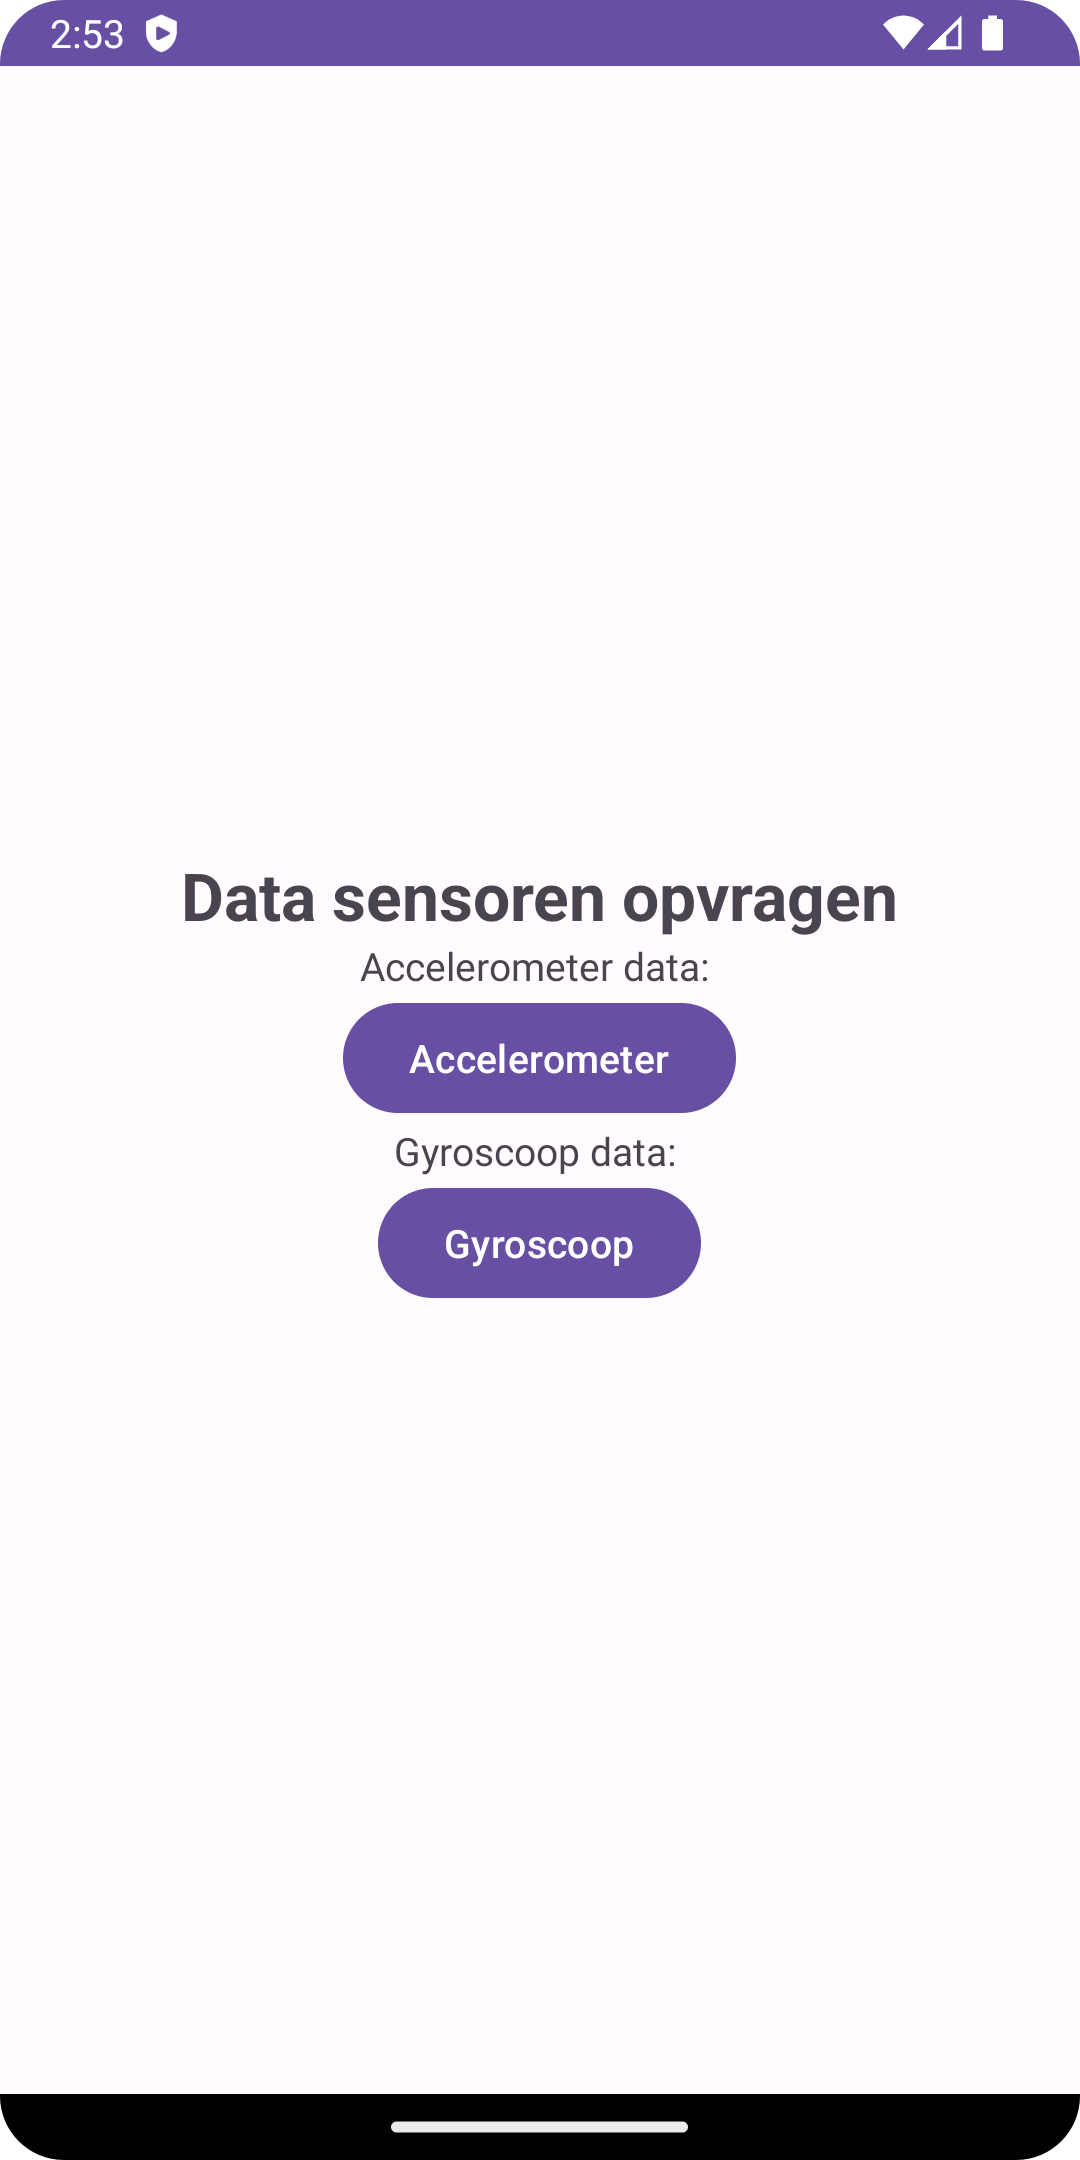
\includegraphics[height=0.5\textheight]{sensoren_layoutnative.png}
    \caption{Layout van applicatie voor data van sensoren op te halen bij Android.}
\end{figure}

\subsubsection{Ontwikkeltijd}

Aangezien dat er geen extra libraries of tools gebruikt worden om de sensoren te gebruiken, 
kunnen de sensoren snel geïmplementeerd worden. Enkel moeten de juiste 
permission worden toegevoegd aan het AndroidManifest.xml bestand, de juiste klasse moet geïmporteerd worden en de juiste 
methode moet worden aangeroepen. Daarom is de tijd nodig om de sensoren te gebruiken dus zeer laag. 
Er is ongeveer 45 minuten gespendeerd om de sensoren te implementeren, inclusief opzoekwerk. Er zijn ook geen grote problemen of 
bugs voorgekomen tijdens de implementatie.




\subsubsection{Performantie}

\paragraph{Tijdsduur}
\begin{figure}[H]
    \centering
    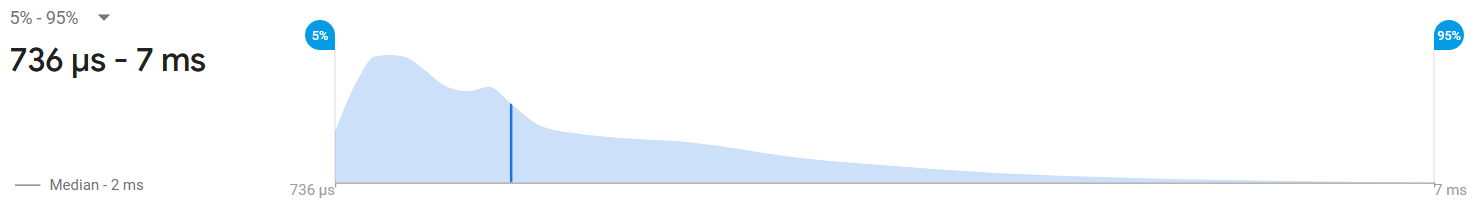
\includegraphics[height=0.085\textheight]{sensorenDuratieNativeAccelerometer.png}
    \caption{Overzicht tijdsduur ophalen van accelerometer data bij Android.}
\end{figure}
Van zodra er op de knop wordt gedrukt om gegevens op te halen van de accelerometer blijft de applicatie
dit continu doen. Hierdoor worden er honderden metingen gedaan die ons vertellen dat het ophalen 
van de accelerometer data gemiddeld 2ms duurt. De minimum en maximum waarden liggen op 736µs en 7ms.
\begin{figure}[H]
    \centering
    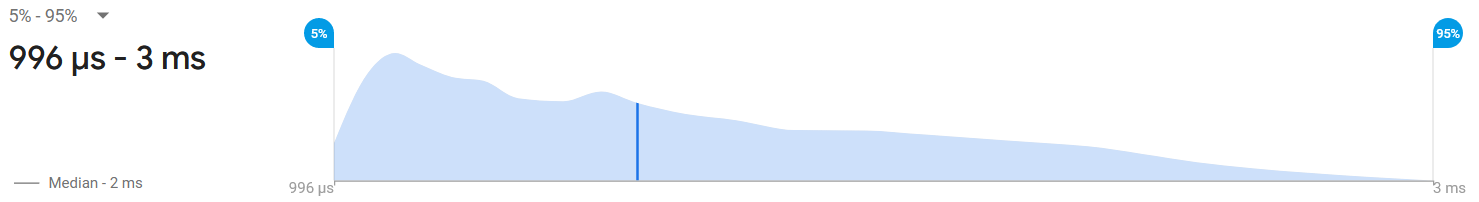
\includegraphics[height=0.085\textheight]{sensorenDuratieNativeGyroscoop.png}
    \caption{Overzicht tijdsduur ophalen van gyroscoop data bij Android.}
\end{figure}
Net zoals bij de accelerometer worden er constant gegevens opgehaald van zodra er op de knop wordt gedrukt. 
Hierdoor worden er opnieuw honderden metingen gedaan die ons vertellen dat het ophalen 
van de gyroscoop data gemiddeld 2ms duurt. De minimum en maximum waarden liggen op 996µs en 3ms.

\paragraph{CPU \& geheugen}
\begin{figure}[H]
    \centering
    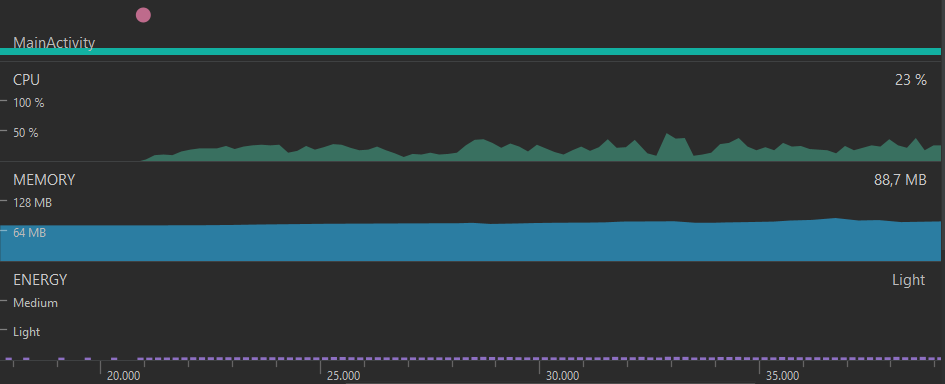
\includegraphics[height=0.25\textheight]{sensorenPerformantieNativeAccelerometer.png}
    \caption{Overzicht CPU en geheugen gebruik tijdens het ophalen van accelerometer data bij Android.}
\end{figure}
Op de grafiek is te zien dat het CPU gebruik van de applicatie bij het ophalen van de accelerometer data,
gemiddeld 23\% is met toch wel redelijke schommelingen. Wanneer er nog geen data wordt opgehaald, wordt de CPU niet 
gebruikt. Het geheugen blijft rond de 88MB hangen, met verschillen van maximum 4-5MB. 
Er is geen merkbaar verschil in het geheugen wanneer er data wordt opgehaald of wanneer er 
geen data wordt opgehaald.
\begin{figure}[H]
    \centering
    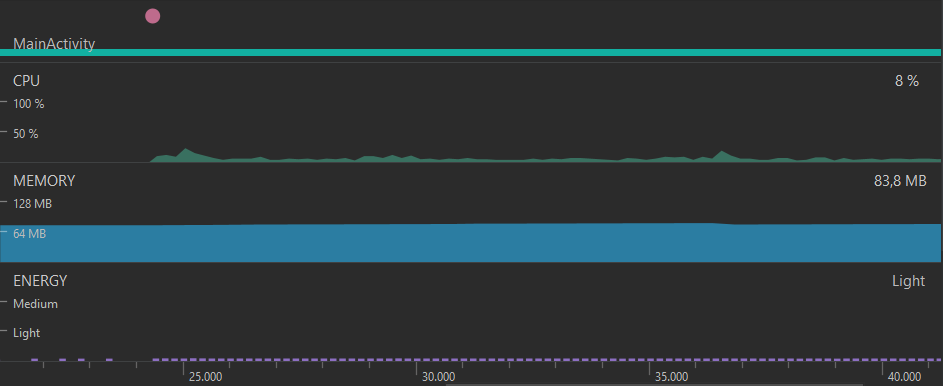
\includegraphics[height=0.25\textheight]{sensorenPerformantieNativeGyroscoop.png}
    \caption{Overzicht CPU en geheugen gebruik tijdens het ophalen van gyroscoop data bij Android.}
\end{figure}
Net zoals bij de accelerometer is op de grafiek te zien dat het CPU gebruik van de applicatie bij het 
ophalen van de gyroscoop data, gemiddeld 8\% is. Wat opvalt, is dat er bij het ophalen van de gyroscoop data
in het begin een piek is van 30\%. Maar dat dit daarna terug zakt naar 8\%. Bij de accelerometer was er geen
piek te zien maar was het gemiddelde CPU gebruik wel hoger. Net zoals bij de accelerometer is er ook geen 
CPU gebruik wanneer er geen data wordt opgehaald. Het geheugen blijft terug rond de 88MB hangen, met 
verschillen van maximum 4-5MB. Opnieuw is er geen merkbaar verschil in het 
geheugen wanneer er data wordt opgehaald of wanneer er geen data wordt opgehaald.
  


\subsubsection{Schaalbaarheid}

\paragraph{Complexiteit}
Het proces om de data van sensoren te verkrijgen is vrij simpel. De ontwikkelaar moet enkel de juiste klasse importeren, 
de juiste methode aanroepen en de juiste permissies toevoegen aan de AndroidManifest.xml file. Indien dat er iets niet 
duidelijk is, is er altijd de documentatie van Android waarin alles duidelijk wordt uitgelegd.

\paragraph{Herbruikbaarheid}
Het is gemakkelijk om de gegevens van de sensoren te hergebruiken. We kunnen bijvoorbeeld in plaats van de 
gegevens in een TextView component te tonen, de gegevens in een object opslaan. Dat object kan dan vanuit 
een andere klasse worden opgevraagd. Het is ook mogelijk om de logica voor het ophalen van de gegevens
in een aparte klasse te plaatsen. Zo kan de logica gemakkelijk worden hergebruikt in andere klassen. 
En kan deze ook aangepast of opgeschaald worden.



\section{Cross-platform}
\subsubsection{Wat is er nodig}
Om bij React Native toegang te krijgen tot de sensoren moet er gebruik worden gemaakt van de react-native-sensors library.
Deze library biedt onder andere toegang tot de accelerometer en gyroscoop. Het is een wrapper voor de
native sensoren van Android en iOS. 

\subsubsection{Uitvoering}

\paragraph{1. Library toevoegen}
Als eerst voegen we React Native Sensors toe aan de root van ons project.
\begin{minted}{bash}
npm install react-native-sensors --save
\end{minted}

\paragraph{2. Package teruggeven}
Normaal gezien moeten we de package dan toevoegen aan het 
\textit{android/app/src/} \textbf{main/java/com/project/MainApplication.java} bestand.
Maar dit is niet meer nodig bij React Native 0.60+.

\paragraph{3. gradle instellingen aanpassen}
Tot slot voegen we de volgende regel toe aan het \textit{android/app/build.gradle} bestand.
\begin{minted}{groovy}
implementation project(':react-native-sensors')
\end{minted}
En voegen we de volgende regel toe aan het \textit{android/settings.gradle} bestand.
\begin{minted}{groovy}
include ':react-native-sensors'
project(':react-native-sensors').projectDir = 
    new File(rootProject.projectDir
        , '../node_modules/react-native-sensors/android')
\end{minted}
De package is nu volledig geïnstalleerd en klaar voor gebruik.

\paragraph{4. Sensor gebruiken}
Eerst importeren we de library in het bestand waar we deze nodig hebben.
\begin{minted}{typescript}
import { accelerometer, gyroscope } from "react-native-sensors";
\end{minted}
Daarna definiëren we twee variabelen die de data van de sensoren zal bewaren.
\begin{minted}{typescript}
const [accelerometerData, setAccelerometerData] = useState({});
const [gyroscopeData, setGyroscopeData] = useState({});
\end{minted}
Tot slot kunnen we dan deze variabelen gebruiken om de data van de sensoren op te vragen.
\begin{minted}{typescript}
const getData = () => {
    setIsFetchingData(true);

    startFetchingData();
};

const startFetchingData = () => {
    if (isFetchingData) {
        const accelerometerSubscription = new Accelerometer({
            updateInterval: 100, // Verander dit indien nodig
        }).subscribe(({ x, y, z }) => {
            // Doe iets met de accelerometerwaarden (x, y, z)
        });

        const gyroscopeSubscription = new Gyroscope({
        updateInterval: 100, // Verander dit indien nodig
        }).subscribe(({ x, y, z }) => {
            // Doe iets met de accelerometerwaarden (x, y, z)
        });

        // Unsubscribe van de sensoren wanneer je klaar bent 
        // met het ophalen van de data
        return () => {
            accelerometerSubscription.unsubscribe();
            gyroscopeSubscription.unsubscribe();
        };
    }
};
\end{minted}

\paragraph{4. Applicatie maken}
Net zoals bij de native applicatie maken we een applicatie die de accelerometer en gyroscoop data 
opvraagt en weergeeft. Deze bestaat uit twee \textbf{<Text>} componenten voor de data van de
accelerometer en gyroscoop weer te geven en tot slot twee \textbf{<Button>} componenten om de 
data op te halen. Als de knoppen ingedrukt worden, dan wordt ofwel de
\textbf{onPress} of \textbf{onPress} methode aangeroepen. In deze methodes wordt de data 
van de sensoren opgehaald en in de \textbf{<Text>} componenten geplaatst.
\begin{figure}[H]
    \centering
    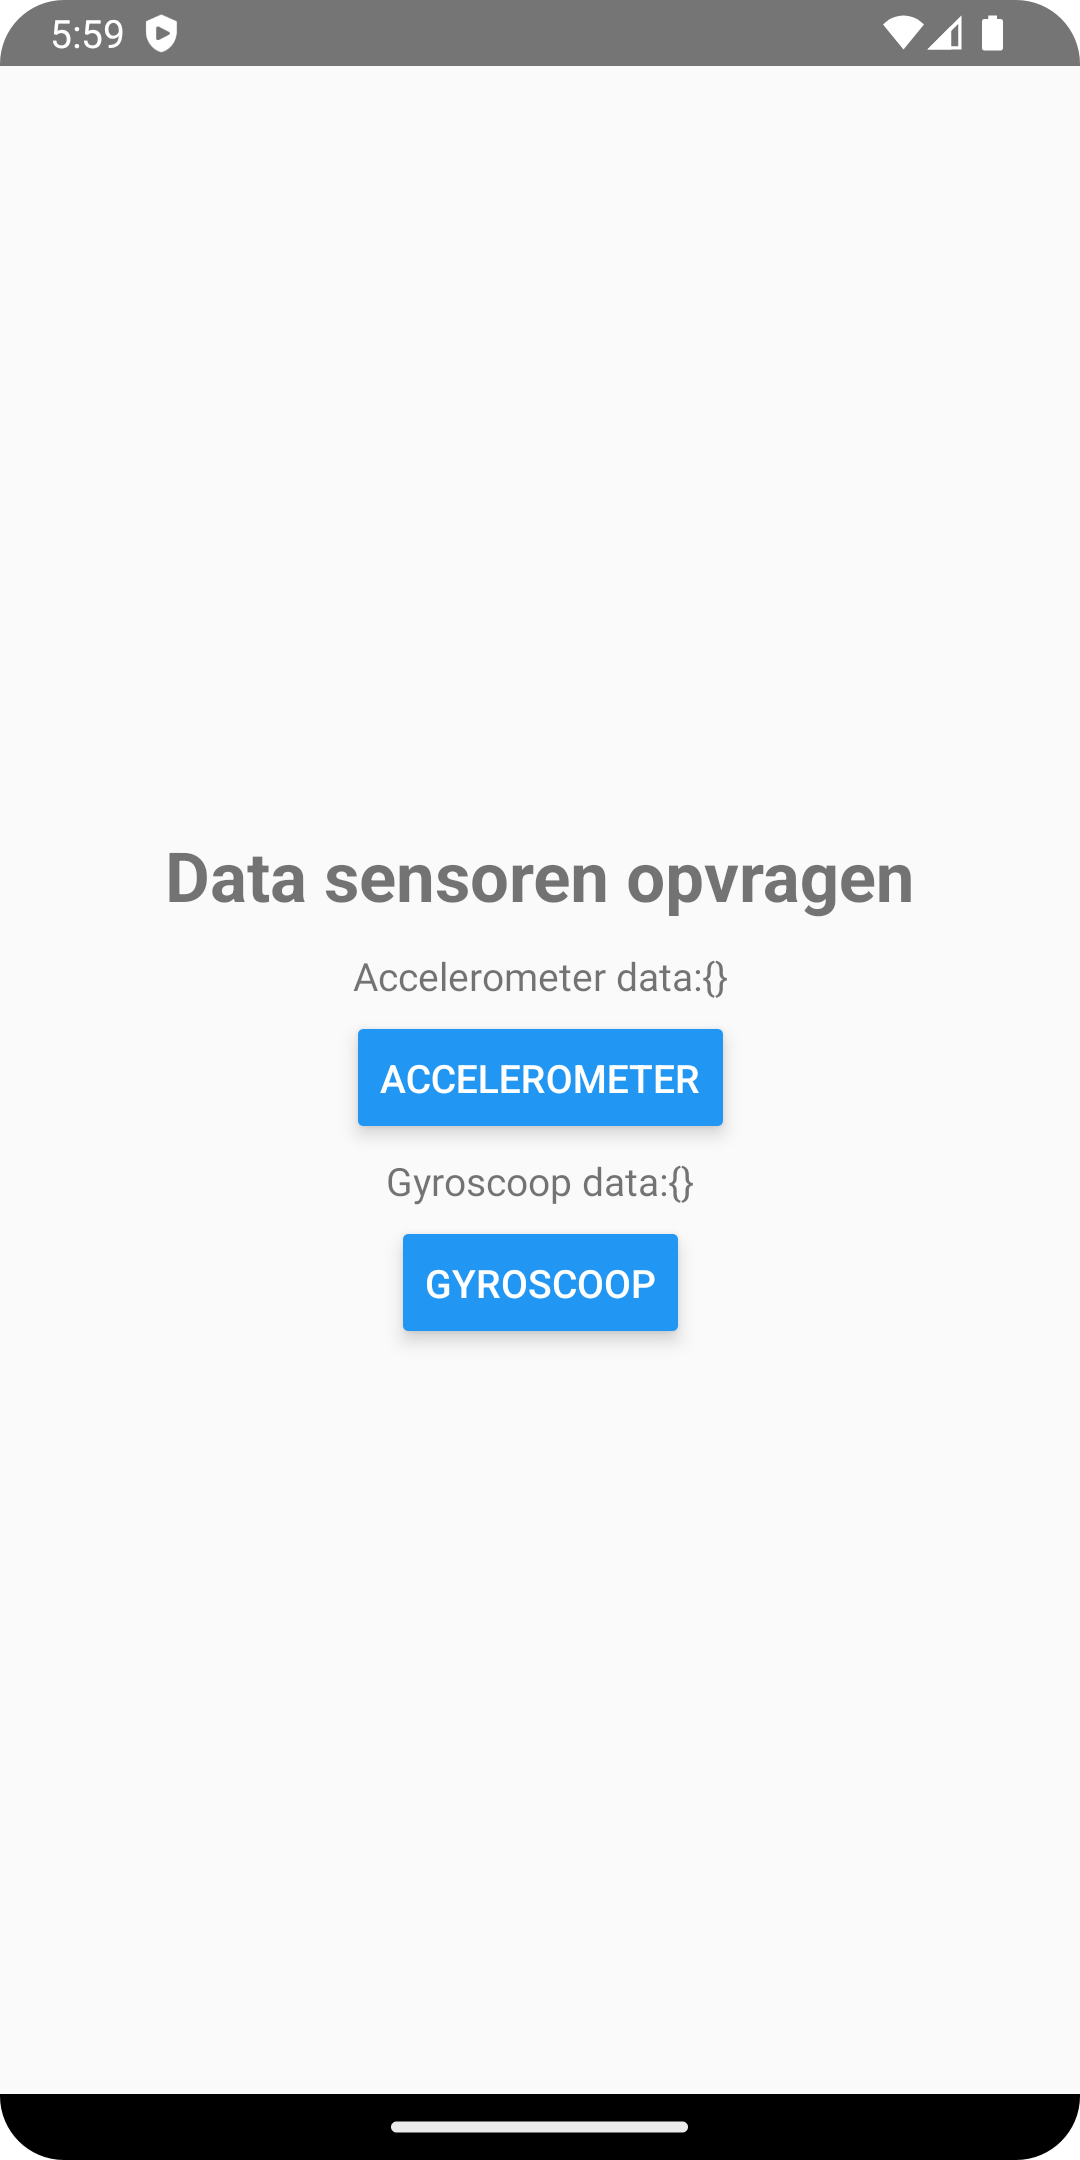
\includegraphics[height=0.4\textheight]{sensoren_layoutcross.png}
    \caption{Layout van applicatie voor data van sensoren op te halen bij React Native.}
\end{figure}

\subsubsection{Ontwikkeltijd}

In vergelijking met native ontwikkeling, moeten er wel meer stappen ondernomen worden om de 
sensoren te gebruiken. Eerst en vooral moet er een externe library geïmplementeerd worden 
om de sensoren te gebruiken. Pas daarna kunnen de sensoren worden gebruikt. Daardoor is de tijd die nodig
was om de sensoren te gebruiken hoger dan bij native ontwikkeling. We hebben ongeveer
1 uur en 15 minuten gespendeerd om de sensoren te gebruiken. Er zijn ook geen grote problemen of
bugs voorgekomen tijdens de implementatie.


\subsubsection{Performantie}

\paragraph{Tijdsduur}
\begin{figure}[H]
    \centering
    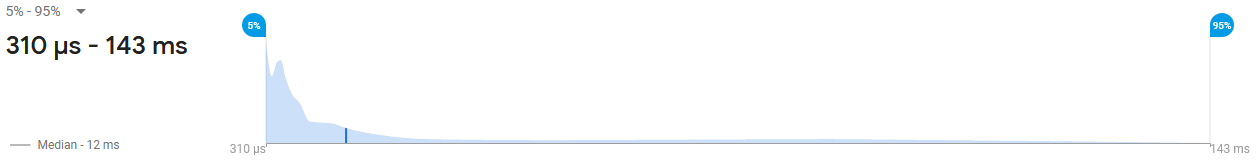
\includegraphics[height=0.1\textheight]{sensorenDuratieCrossAccelerometer.png}
    \caption{Overzicht tijdsduur ophalen van accelerometer data bij React native.}
\end{figure}


\begin{figure}[H]
    \centering
    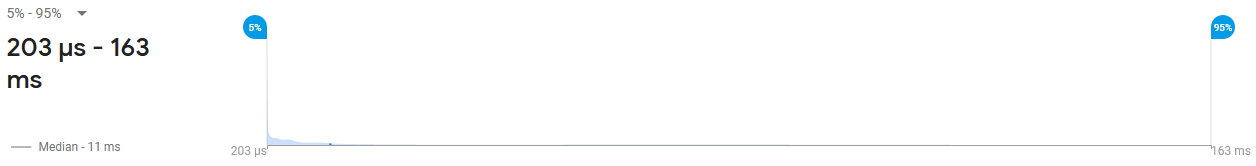
\includegraphics[height=0.1\textheight]{sensorenDuratieCrossGyroscoop.png}
    \caption{Overzicht tijdsduur ophalen van gyroscoop data bij React native.}
\end{figure}


\paragraph{CPU \& geheugen}
\begin{figure}[H]
    \centering
    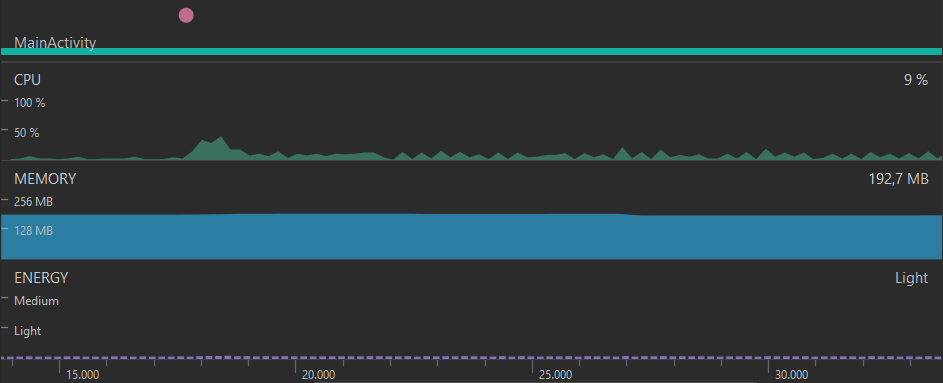
\includegraphics[height=0.3\textheight]{sensorenPerformantieCrossAccelerometer.png}
    \caption{Overzicht CPU en geheugen gebruik tijdens het ophalen van accelerometer data bij React native.}
\end{figure}


\begin{figure}[H]
    \centering
    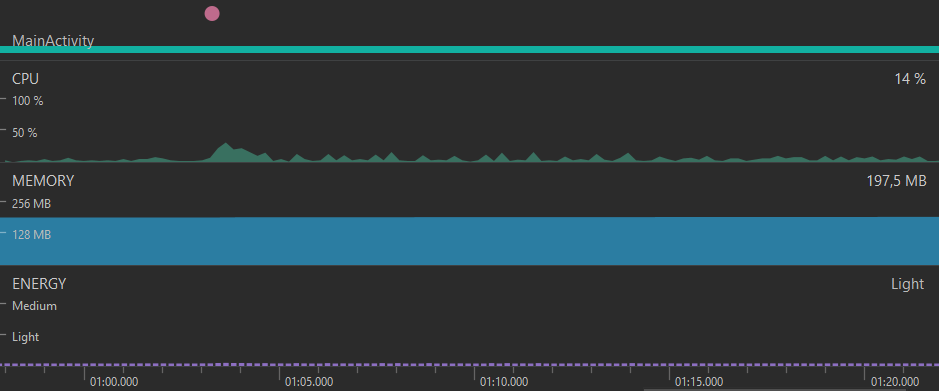
\includegraphics[height=0.3\textheight]{sensorenPerformantieCrossGyroscoop.png}
    \caption{Overzicht CPU en geheugen gebruik tijdens het ophalen van gyroscoop data bij React native.}
\end{figure}


\subsubsection{Schaalbaarheid}

\paragraph{Complexiteit}
Het gebruiken van de sensoren is net zoals bij native vrij simpel. Ondanks dat er een extra library moet worden
geïmplementeerd. De package zorgt ervoor dat het ophalen van de data van de sensoren overeenkomt met het 
ophalen van de data van de sensoren bij native. Daarnaast is er ook net zoals bij native de documentatie van
de library die alles duidelijk uitlegt.

\paragraph{Herbruikbaarheid}
Net zoals bij native is het makkelijk om de gegevens van de sensoren te hergebruiken. We kunnen bijvoorbeeld in plaats van de
gegevens in een useState hook te plaatsen, de gegevens in een globale variabel of in een useContext opslaan. 
Om dan in andere componenten de gegevens op te vragen. Het is ook mogelijk om de logica voor het ophalen van de gegevens
in een aparte useContext te plaatsen. Zo kan de logica makkelijk worden hergebruikt in andere componenten.
En kan deze ook aangepast of opgeschaald worden. 



\section{Conclusie}
De tijdsduur van het ophalen van de data van de sensoren is bij native veel sneller dan bij cross-platform.
Dit komt omdat de library die gebruikt wordt bij cross-platform een wrapper is voor de native sensoren.
Hierdoor moet de data van de sensoren eerst naar de wrapper gestuurd worden en pas daarna naar de applicatie.
Bij native is dit niet het geval: de data van de sensoren wordt rechtstreeks naar de applicatie gestuurd.
Het ophalen van data is daardoor gemiddeld 10ms trager bij cross-platform dan bij native.
\\\\
Bij het geheugengebruik is er geen verschil tijdens het ophalen van sensoren data en evenmin wanneer er 
niks gebeurt in de applicatie. Ondanks het feit dat het ophalen van data niet beïnvloed 
wordt, wordt er 121.59\% meer geheugen gebruikt bij React Native dan 
bij Android (88MB in vergelijking met gemiddeld 195MB). Dit komt omdat cross-platform een extra 
library moet implementeren. Deze library neemt ook geheugen in beslag.
\\\\
Bij het CPU gebruik zijn er onderling tussen de accelerometer en gyroscoop ook verschillen. Bij native 
heeft de accelerometer geen piek maar blijft deze constant op gemiddeld 23\% CPU gebruik. Bij cross-platform heeft
de accelerometer een piek van 50\% CPU gebruik waarna deze naar 9\% zakt, een groot verschil. 
De gyroscoop heeft bij native een piek 30\% CPU gebruik waarna deze naar 8\% zakt. Bij cross-platform
is de piek 40\% CPU gebruik waarna deze naar 10\% zakt. Daarnaast is er bij alle sensoren een schommeling van 5 tot 20\%. 
Dit komt omdat de sensoren data constant wordt opgehaald. Normaal zou er verwacht worden dat de sensoren bij native 
minder CPU gebruiken, aangezien de data eerst naar de wrapper wordt gestuurd en pas daarna naar de applicatie. Maar bij 
de accelerometer is dit niet het geval. Hier is het CPU gebruik bij cross-platform lager dan bij native.
\\\\
\begin{tabular}{ |p{3cm}||p{5cm}|p{5cm}| }
    \hline
    \multicolumn{3}{|c|}{Accelerometer} \\ 
    \hline
     & Native (Android) & Cross-platform (React Native) \\
    \hline
     & \multicolumn{2}{|c|}{Tijdsduur} \\
    \hline
    Minimaal & 736µs & 310µs \\
    Maximaal & 7ms & 143ms \\
    Gemiddeld & 2ms & 12ms \\
    \hline
     & \multicolumn{2}{|c|}{Geheugen} \\ 
    \hline
    Offset & 2-3MB & 3-4MB \\
    Gemiddeld & 88MB & 192MB \\
    \hline
     & \multicolumn{2}{|c|}{CPU} \\
    \hline
    (Begin)Piek & / & 50\% \\
    Offset & 20\% & 10\% \\
    Gemiddeld & 23\% & 9\% \\
    \hline
\end{tabular}
\\\\
\begin{tabular}{ |p{3cm}||p{5cm}|p{5cm}| }
    \hline
    \multicolumn{3}{|c|}{Gyroscoop} \\ 
    \hline
     & Native (Android) & Cross-platform (React Native) \\
    \hline
     & \multicolumn{2}{|c|}{Tijdsduur} \\
    \hline
    Minimaal & 996µs & 203µs \\
    Maximaal & 3ms & 163ms \\
    Gemiddeld & 2ms & 11ms \\
    \hline
     & \multicolumn{2}{|c|}{Geheugen} \\ 
    \hline
    Offset & 4-5MB & 3-4MB \\
    Gemiddeld & 88MB & 197MB \\
    \hline
     & \multicolumn{2}{|c|}{CPU} \\
    \hline
    (Begin)Piek & 30\% & 40\% \\
    Offset & 5\% & 10\% \\
    Gemiddeld & 8\% & 10\% \\
    \hline
\end{tabular}
\\\\
De ontwikkeltijd voor het implementeren van sensoren
bij native en cross-platform is ongeveer hetzelfde. Buiten het feit dat cross-platform een extra library moet
implementeren waardoor de ontwikkeltijd iets langer wordt. 
\\\\
Op vlak van schaalbaarheid is er geen verschil tussen native en cross-platform. Beide applicaties kunnen
gemakkelijk uitgebreid worden met extra sensoren en de bestaande logica van de sensoren kan gemakkelijk 
hergebruikt of opgeschaald worden.
\\\\
Uit deze resultaten kan geconcludeerd worden dat applicaties die intensief gebruik maken van de sensoren 
beter native gebruiken aangezien deze sneller gegevens kan ophalen. Daarnaast is cross-platform beter in gebruik 
voor eenvoudige applicaties die de sensoren niet intensief gebruiken.














